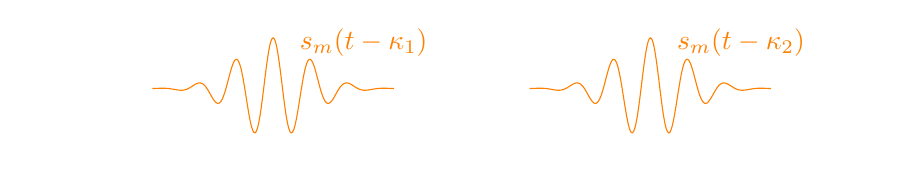
\begin{tikzpicture}[/pgfplots/.cd,width=\columnwidth,height=3cm]
    \begin{axis}[xmin=-0.5,xmax=5,ymin=-1,ymax=1.2,
        xticklabels=\empty,
        yticklabels=\empty,
        axis line style={draw=none},
        tick style={draw=none}]
        %\addplot[no markers,smooth,samples=201,domain=0:2.5, color=white] 
        {exp(-9*(x-1)*(x-1))*cos((x-1)*1440)};

        %\addplot[no markers,smooth,samples=401,domain=0:5, color=white] 
        %{exp(-9*(x-1)*(x-1))*cos((x-1)*1440) + exp(-9*(x-3.5)*(x-3.5))*cos((x-3.5)*1440)};
        %\addplot[no markers,smooth,samples=201,domain=0.2:1.8, color=orange] 
        {exp(-9*(x-1)*(x-1))*cos((x-1)*1440)};
        %\addplot[no markers,smooth,samples=201,domain=2.7:4.3, color=orange] 
        {exp(-9*(x-3.5)*(x-3.5))*cos((x-3.5)*1440)};
        % 

        \addplot[no markers,smooth,samples=2,domain=0:0.2, color=white]
        {exp(-9*(x-1)*(x-1))*cos((x-1)*1440) + exp(-9*(x-3.5)*(x-3.5))*cos((x-3.5)*1440)}; 
        \addplot[no markers,smooth,samples=201,domain=0.2:1.8, color=orange]
        {exp(-9*(x-1)*(x-1))*cos((x-1)*1440) + exp(-9*(x-3.5)*(x-3.5))*cos((x-3.5)*1440)};
        \addplot[no markers,smooth,samples=2,domain=1.8:2.7, color=white]
        {exp(-9*(x-1)*(x-1))*cos((x-1)*1440) + exp(-9*(x-3.5)*(x-3.5))*cos((x-3.5)*1440)};
        \addplot[no markers,smooth,samples=201,domain=2.7:4.3, color=orange]
        {exp(-9*(x-1)*(x-1))*cos((x-1)*1440) + exp(-9*(x-3.5)*(x-3.5))*cos((x-3.5)*1440)};
        \addplot[no markers,smooth,samples=2,domain=4.3:5, color=white]
        {exp(-9*(x-1)*(x-1))*cos((x-1)*1440) + exp(-9*(x-3.5)*(x-3.5))*cos((x-3.5)*1440)};

        {exp(-9*(x-1)*(x-1))*cos((x-1)*1440) + exp(-9*(x-3.5)*(x-3.5))*cos((x-3.5)*1440)};


        \node[text=orange] at (axis cs:1.6,0.9) {$s_m(t-\kappa_1)$};
        \node[text=orange] at (axis cs:4.1,0.9) {$s_m(t-\kappa_2)$};
        \node[color=white] at (axis cs:-0.1,0.4) {$y_m(t)$};

        %\node[color=white] at (axis cs:0.2,-0.3) {$ $};
        %\node[] at (axis cs:0.2,0) {$|$};
        %\node[] at (axis cs:1.8,0) {$|$};
        %\node[color=white] at (axis cs:2.7,-0.3) {$ $};
        %\node[] at (axis cs:2.7,0) {$|$};
        %\node[] at (axis cs:4.3,0) {$|$};

    \end{axis}
\end{tikzpicture}

\begin{tikzpicture}[/pgfplots/.cd,width=\columnwidth,height=3cm]
    \begin{axis}[xmin=-0.5,xmax=5,ymin=-1,ymax=1.2,
        xticklabels=\empty,
        yticklabels=\empty,
        axis line style={draw=none},
        tick style={draw=none}]
        \addplot[no markers,smooth,samples=201,domain=0:2.5, color=white] 
        {exp(-9*(x-1)*(x-1))*cos((x-1)*1440)};

        \addplot[no markers,smooth,samples=201,domain=2.5:5, color=white] 
        {exp(-9*(x-3.5)*(x-3.5))*cos((x-3.5)*1440)};
        \addplot[no markers,smooth,samples=201,domain=0.2:1.8, color=orange] 
        {exp(-9*(x-1)*(x-1))*cos((x-1)*1440)};
        %\addplot[no markers,smooth,samples=201,domain=2.7:4.3, color=orange] 
        {exp(-9*(x-3.5)*(x-3.5))*cos((x-3.5)*1440)};
        % 
        \node[text=orange] at (axis cs:1.6,0.9) {$s_m(t-\kappa_1)$};
        %\node[text=orange] at (axis cs:4.1,0.9) {$s_m(t-\kappa_2)$};
        \node[color=white] at (axis cs:-0.1,0.4) {$y_m(t)$};

        \node[color=white] at (axis cs:0.2,-0.3) {$ $};
        \node[color=white] at (axis cs:0.2,0) {$|$};
        \node[color=white] at (axis cs:2.7,-0.3) {$ $};
        %\node[] at (axis cs:2.7,0) {$|$};
    \end{axis}
\end{tikzpicture}

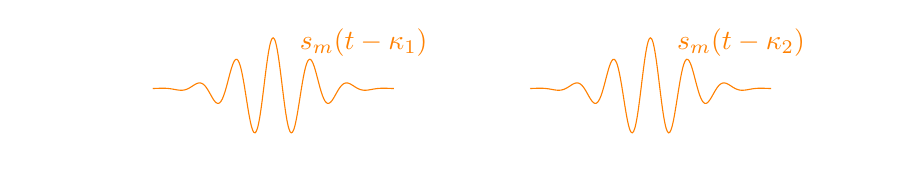
\begin{tikzpicture}[/pgfplots/.cd,width=\columnwidth,height=3cm]
    \begin{axis}[xmin=-0.5,xmax=5,ymin=-1,ymax=1.2,
        xticklabels=\empty,
        yticklabels=\empty,
        axis line style={draw=none},
        tick style={draw=none}]
        \addplot[no markers,smooth,samples=201,domain=0:2.5, color=white] 
        {exp(-9*(x-1)*(x-1))*cos((x-1)*1440)};

        \addplot[no markers,smooth,samples=201,domain=2.5:5, color=white] 
        {exp(-9*(x-3.5)*(x-3.5))*cos((x-3.5)*1440)};
        \addplot[no markers,smooth,samples=201,domain=0.2:1.8, color=orange] 
        {exp(-9*(x-1)*(x-1))*cos((x-1)*1440)};
        \addplot[no markers,smooth,samples=201,domain=2.7:4.3, color=orange] 
        {exp(-9*(x-3.5)*(x-3.5))*cos((x-3.5)*1440)};
        % 
        \node[text=orange] at (axis cs:1.6,0.9) {$s_m(t-\kappa_1)$};
        \node[text=orange] at (axis cs:4.1,0.9) {$s_m(t-\kappa_2)$};
        \node[color=white] at (axis cs:-0.1,0.4) {$y_m(t)$};

        \node[color=white] at (axis cs:0.2,-0.3) {$ $};
        \node[color=white] at (axis cs:0.2,0) {$|$};
        \node[color=white] at (axis cs:2.7,-0.3) {$ $};
        \node[color=white] at (axis cs:2.7,0) {$|$};
    \end{axis}
\end{tikzpicture}